\documentclass[border=6pt]{standalone}
\usepackage[T1]{fontenc}\usepackage{lmodern}\usepackage{amsmath,amssymb}\usepackage{xcolor}\usepackage{tikz}
\usetikzlibrary{arrows.meta,positioning,calc,fit,shapes.misc}
% TikZ styles
\tikzset{
  blk/.style={draw, rounded corners=2pt, align=center, font=\small, minimum height=8mm, inner sep=4pt, fill=#1},
  blk/.default=white,
  arr/.style={-{Stealth[length=2.2mm]}, thick},
}
\definecolor{base}{HTML}{FBE3E3}
\definecolor{prop}{HTML}{DDEBFA}
\definecolor{same}{HTML}{EDEDED}
\definecolor{done}{HTML}{DFF1DF}
\definecolor{todo}{HTML}{FFF2CC}

\begin{document}
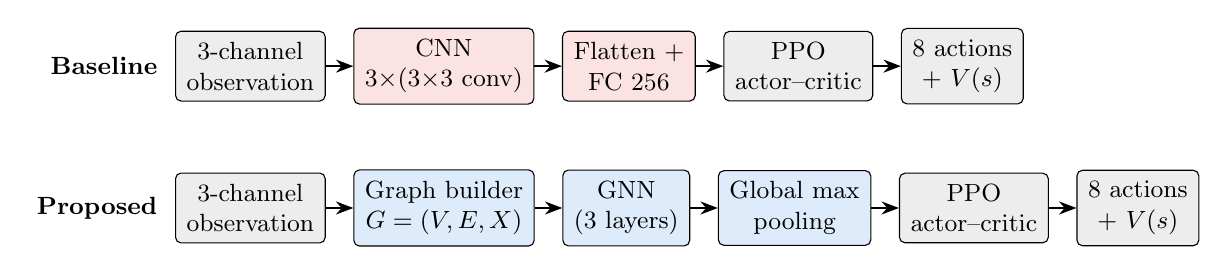
\begin{tikzpicture}[node distance=3.5mm and 3.5mm]
  \node[blk=same] (o1) {3-channel\\observation};
  \node[blk=base, right=of o1] (c1) {CNN\\3$\times$(3$\times$3 conv)};
  \node[blk=base, right=of c1] (f1) {Flatten +\\FC 256};
  \node[blk=same, right=of f1] (p1) {PPO\\actor--critic};
  \node[blk=same, right=of p1] (a1) {8 actions\\$+\ V(s)$};
  \foreach \u/\v in {o1/c1,c1/f1,f1/p1,p1/a1} \draw[arr] (\u) -- (\v);
  \node[left=1mm of o1, font=\small\bfseries, anchor=east] {Baseline};

  \node[blk=same, below=9mm of o1] (o2) {3-channel\\observation};
  \node[blk=prop, right=of o2] (g2) {Graph builder\\$G=(V,E,X)$};
  \node[blk=prop, right=of g2] (n2) {GNN\\(3 layers)};
  \node[blk=prop, right=of n2] (m2) {Global max\\pooling};
  \node[blk=same, right=of m2] (p2) {PPO\\actor--critic};
  \node[blk=same, right=of p2] (a2) {8 actions\\$+\ V(s)$};
  \foreach \u/\v in {o2/g2,g2/n2,n2/m2,m2/p2,p2/a2} \draw[arr] (\u) -- (\v);
  \node[left=1mm of o2, font=\small\bfseries, anchor=east] {Proposed};
\end{tikzpicture}
\end{document}
